\section{Image-based rendering - extended plane sweeping}

% \begin{figure*}[htbp]
% \centerline{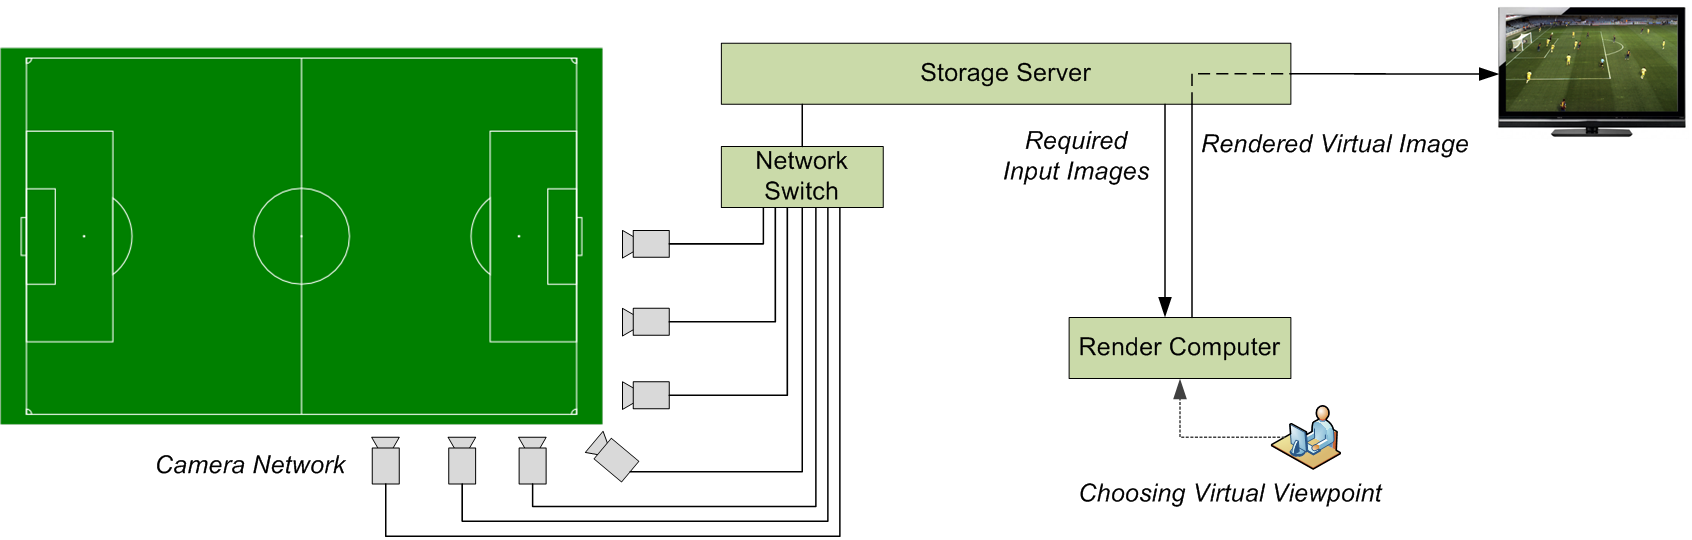
\includegraphics[scale=0.18]{plane_sweeping.png}}
% \caption{TODO}
% \label{fig:plane_sweeping}
% \end{figure*}

\begin{figure*}[htbp]
\centerline{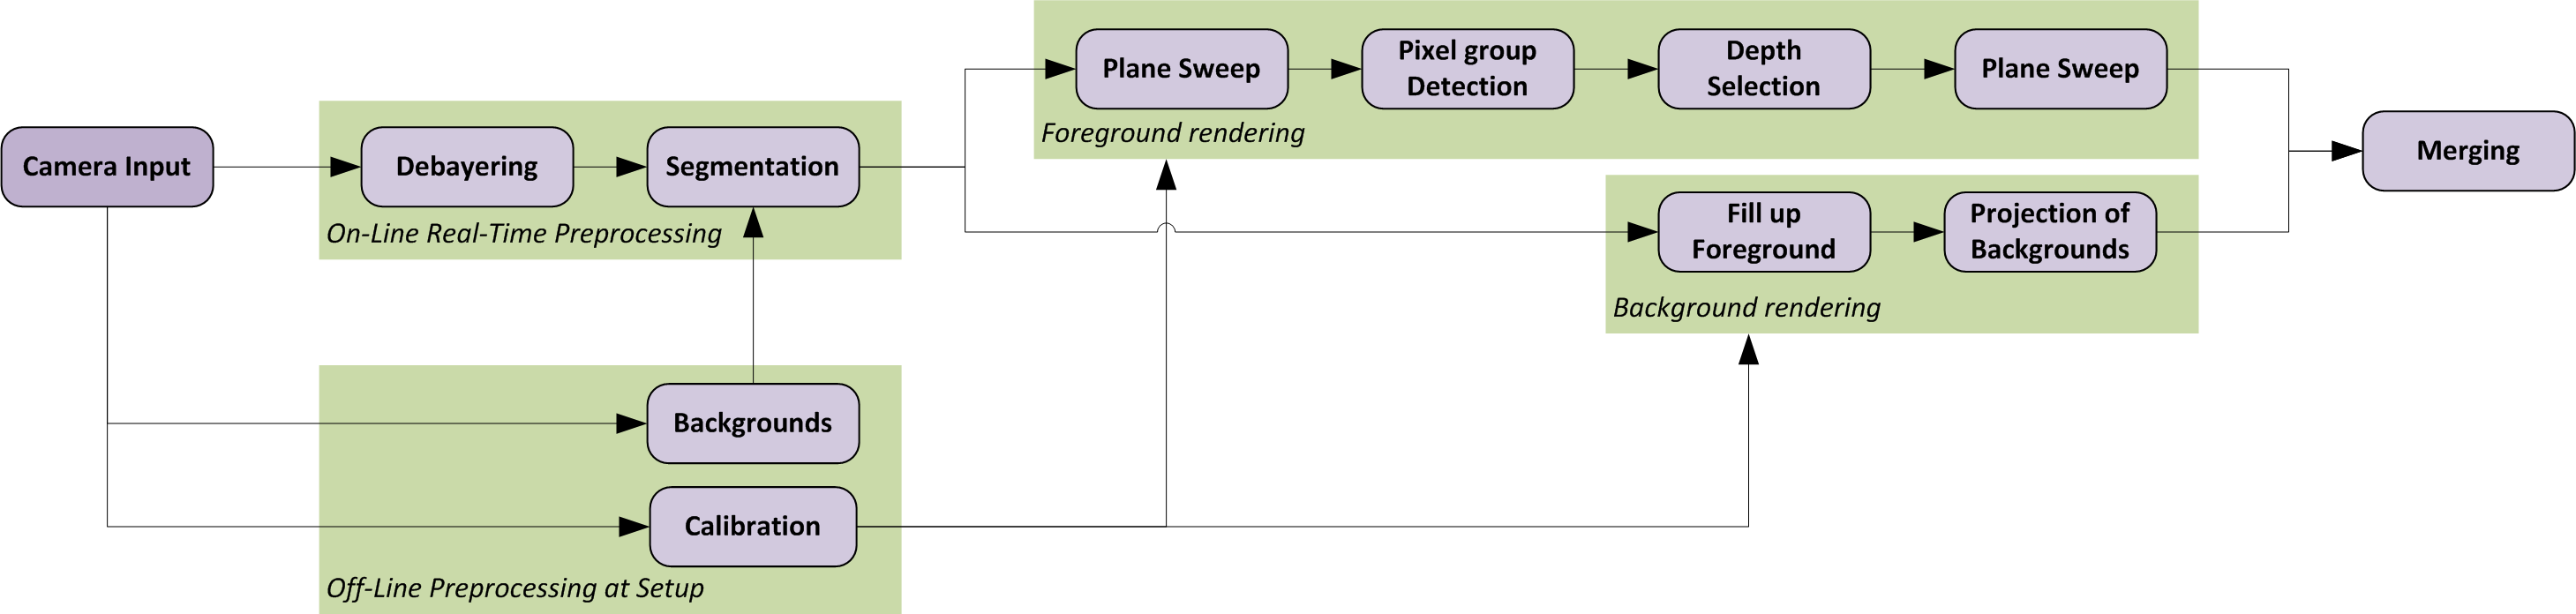
\includegraphics[scale=0.18]{plane_sweeping2.png}}
\caption{TODO}
\label{fig:plane_sweeping2}
\end{figure*}

In this section we present the work of Goorts et al. \cite{plane_sweeping}, an image-based approach to generate 
virtual camera images interpolating real camera images.
Instead of performing 3D reconstruction, image-based methods generate directly the image of the novel viewpoint.
When multiple cameras are present, plane sweeping can be used [05:Yang et al., 2004] for both small and wide 
baseline setups.
Plane sweeping has already been used for novel view point in soccer scenes. Goorts et al. [05:Goorts
et al., 2012a; Goorts et al., 2013a] present a method
with two plane sweeps and a depth filtering step suitable for smaller baseline 
setups of about 1 meter. 
This method present some problems like disappearing players
when they overlap in the image.

The method presented here is fully automatic and employ GPU
parallel processing to achieve fast processing speed.
The system setup consists of 7 static cameras placed in a
wide baseline setup, i.e. 10 meters between each camera.
All cameras are synchronized on shutter level using a global clock.
% All images are transferred to a storage server,
% where all the captured data is stored. A render com-
% puter can access all required images to generate a
% novel viewpoint.
The generation of novel viewpoint consists of two steps as shown in Figure \ref{fig:plane_sweeping2}:
a first off-line preprocessing phase and a real-time interpolation phase. 
As explained in \cite{plane_sweeping}, the preprocessing phase is responsible of camera
calibration, acquiring position, orientation and intrinsic parameters for each camera, and background determination. 
The real-time phase generates images for a chosen virtual camera 
position and a chosen time in the video sequence.
More in details, camera images are debayered and segmented using GPUs.
Debayering consists of converting the raw images to its RGB representation and segmentation is based on backgrounds
obtained during off-line preprocessing.
This method \cite{plane_sweeping} allows fast segmentation in high quality.
These images are then used to process foreground and background independently. 
The foreground rendering uses a plane-sweep
approach followed by depth filtering and a depth-
selective plane sweep as explained in \cite{plane_sweeping}.
In this way, the authors obtained high quality results using wide baseline setup and typical artifacts, such as
ghost players, are removed.
% , where the
% reprojection consistency for different depths is maxi-
% mized, thus generating a novel image and depth map
% simultaneously. However, normal plane sweeping
% does not yield high quality results for soccer scenes
% using a wide baseline setup. Serious artifacts, such as
% ghost players, can be perceived. Therefore, we em-
% ploy a depth selection method where the acceptable
% depths of groups of pixels is determined and used in a
% second, depth-selective plane sweep.
% To demonstrate our method, we obtained images
% from a real soccer match in real conditions. Our
% method outperforms other free viewpoint video sys-
% tems, as demonstrated by the results and the accompa-
% nying video. Typical artifacts, such as ghost players,
% are effectively removed.